\documentclass{beamer}
\usepackage[utf8]{inputenc}
\usepackage[english,russian]{babel}

\usepackage{xcolor}

\usepackage{amsmath,amsfonts,amssymb,amsthm,amscd,amsxtra}
\usepackage{physics}
\usepackage[sharp]{easylist}
\usepackage{comment}
\usepackage{mathtools} % xmapsto, \Vector

\usepackage{beamerthemesplit}
\usetheme{Boadilla}
\setbeamertemplate{caption}[numbered]

% \usepackage[pdftex]{graphicx}
\graphicspath{ {pic/} }
\usepackage{tikz}

\newcommand{\hilb}[1]{\mathcal{H}_{#1}}
\newcommand{\cconj}[1]{\overline{#1}}
\newcommand{\hank}[1]{H_{#1}^{(1)}}

\newcommand{\mcF}{\mathcal{F}}
\newcommand{\mcH}{\mathcal{H}} % ???
\newcommand{\mcI}{\mathcal{I}}
\newcommand{\mcL}{\mathcal{L}} % L2 space
\newcommand{\mcO}{\mathcal{O}} % Big O
\newcommand{\mcP}{\mathcal{P}}


\newcommand{\bbC}{\mathbb{C}} % complex plane
\newcommand{\bbD}{\mathbb{D}} % complex unit disk
\newcommand{\bbH}{\mathbb{H}} % complex upper half-plane TODO add to template
\newcommand{\bbN}{\mathbb{N}}
\newcommand{\bbK}{\mathbb{K}}
\newcommand{\bbR}{\mathbb{R}}
\newcommand{\bbT}{\mathbb{T}} % complex unit circle
\newcommand{\bbZ}{\mathbb{Z}}

\newcommand{\eqdef}{\overset{\mathrm{def}}{=\joinrel=}}

\DeclareMathOperator{\dom}{dom}
\DeclareMathOperator{\ran}{Ran}
\DeclareMathOperator{\rng}{rng}

\newcommand{\todo}[1]{\textcolor{red}{{\large TODO: #1}}}

\newenvironment{elist}{\begin{easylist}[enumerate]}{\end{easylist}}
\newenvironment{ilist}{\begin{easylist}[itemize]}{\end{easylist}}

\newcommand{\myspecial}[1]{\mathrm{#1}}

% imaginary unit
\newcommand{\iu}{{i\mkern1mu}}


\newcommand{\ipcdot}{\ip{\cdot}{\cdot}}
\newcommand{\iip}[2]{[#1,#2]}
\newcommand{\iipcdot}{\iip{\cdot}{\cdot}}

\newcommand{\dsum}{\oplus}
\newcommand{\ddiff}{\ominus}
% indefinite direct sum
\newcommand{\idsum}{[+]}
\newcommand{\iddiff}{[-]}

\DeclarePairedDelimiter{\Vector}{\lparen}{\rparen}

\newcommand{\tit}{\textit}
\newcommand{\cls}{\overline}
\newcommand{\eps}{\varepsilon}


\newcommand{\argmin}{\operatornamewithlimits{argmin}}
\newcommand{\argmax}{\operatornamewithlimits{argmax}}

\renewcommand{\Re}{\operatorname{Re}}
\renewcommand{\Im}{\operatorname{Im}}
\renewcommand{\phi}{\varphi} % TODO is there a prettier way to do that

\newcommand{\eexp}[1]{e^{#1}}

\DeclareMathOperator\atanh{atanh}

% ???
% \newcommand{\abs}[1]{\left| #1 \right|}
% \newcommand{\norm}[1]{\left\lVert #1 \right\rVert}
\newcommand*\Eval[3]{\left.#1\right\rvert_{#2}^{#3}}


\title[]{Исследование полноты резонансных состояний оператора Шредингера
для модели квантовых графов}
\author[Дмитрий Герасимов]{Дмитрий Герасимов\\{\small научный руководитель: \\ д.ф.-м.н., профессор кафедры ВМ, И.Ю.Попов}}
\institute[ИТМО]{Университет ИТМО}
\date{24 мая 2016 года}

\begin{document}

\maketitle

\begin{frame}{TODO!!!!}
Задача исследования полноты важна как в теории, так и на практике.
% Задача полноты важна и с теоретической точки зрения (теория функций, дифференциальные уравнения), так и с практической (возможность разложить состояния в ряд Фурье, аппроксимации и т.п.)

\todo{Картинка с резонатором}

\todo{Картинка с резонатором и проводами}

\todo{Картинка с резонансами, верхняя комплексная плоскость}
\end{frame}

% Рассматривается некий резонатор, оператор Шредингера с граничным условием Дирихле в нем имеет чисто дискретный спектр, набор собственный функций полон в L^2(Omega).
% Далее, рассматриваем возмущение этой задачи, соединяя резонатор с волноводом через небольшое отверстие. После этого дискретный спектр пропадает, а собственные значения «смещаются» в комплексную плоскость и становятся резонансами. Резонансные состояния формально удовлетворяют уравнению Шредингера и граничным условиям, однако не принадлежат L^2(Gamma). С другой стороны, при ограничении их на конечный домен Omega, они лежат в L^2(Omega). 
% Интересным вопросом является нахождение домена, на котором резонансные состояния полны
% Гипотеза: на выпуклой оболочке рассеивателя


% Мы рассматриваем упрощенный вариант: квантовый граф (он же и является своей выпуклой оболочкой)
%  (в случае квантового графа он же ей и является)
% Резонансы являются собственными функциями диссипативного оператора????
% 
% 
% 
% 
% 
% 
% Задача: на каком домене полны резонансные состояния?
\begin{frame}{Существующие результаты}
\begin{figure}
\begin{tikzpicture}[scale=0.5]
\newcommand{\Wglen}{10.0}; % waveguide length

\coordinate (LLL) at (-\Wglen - 1, 0);
\coordinate (RRR) at ( \Wglen + 1, 0);
\coordinate (LL)  at (-\Wglen, 0);
\coordinate (RR)  at ( \Wglen, 0);
% change these to take resonator length into account
\coordinate (L)   at (0, 0);
\coordinate (R)   at (0, 0);
%

\coordinate (U) at (0, 3); % upper point of resonator

% waveguide
\draw[ultra thick, dotted] (LLL) -- (LL);
\draw[ultra thick] (LL)--(L);
\draw[ultra thick] (R)--(RR);
\draw[ultra thick, dotted] (RR) -- (RRR);
%

\draw[<-] (-\Wglen + 1, 2) -- (-\Wglen + 5, 2) node [midway, above] {$R e^{-\iu k x}$};
\draw[->] (-\Wglen + 1, 0.5) -- (-\Wglen + 5, 0.5) node [midway, above] {$e^{\iu k x}$};
\draw[->] (\Wglen - 5, 0.5) -- (\Wglen - 1, 0.5) node [midway, above] {$T e^{\iu k x}$};

\draw[ultra thick] node [below] {$V$} (0, 0) -- node [left] {$\Omega$} (U);
\end{tikzpicture}
\caption{Одномерный резонатор-отрезок с $\delta$-условием в $V$}
\end{figure}


\todo{Трехмерный шар}
\end{frame}


\begin{frame}{Постановка задачи}
% TODO домен оператора Шредингера
Квантовый граф $\Gamma$, состоящий из резонатора $\Omega$ и полубесконечных ребер-волноводов.

Оператор Шредингера $H$ действует как $-\dv[2]{\psi}{x}$ на ребрах.

В вершинах графа — $\delta$-образная потенциальная яма, порождает граничные условия:

\[
\forall i, j \in e(V): \psi_i(V) = \psi_j(V)
\]

\[
\sum\limits_{i \in e(V)} \dv{\psi_i}{x} (V) = a_V \psi(V)
\]

Вопрос: полны ли резонансные состояния на $\Omega$?
\end{frame}


\begin{frame}{Решение задачи на произвольном графе}
\todo{Индукция по количеству ребер?}

\todo{«Стягивание» вершин?}
\end{frame}

\begin{frame}{Резонатор типа «кольцо»}
\todo{картиночка}

\[
\det S = 
\frac
{\cos\left(k\right) + {\left(\frac{a}{2 k} + i\right)} \sin\left(k\right) - 1}
{\cos\left(k\right) + {\left(\frac{a}{2 k} - i\right)} \sin\left(k\right) - 1}
\]

$a = 0$

\todo{формула}

\todo{Отрицательный результат! Полноты нет, $\det S$ уходит в 0 на бесконечности}

\end{frame}

\begin{frame}{Резонатор типа «кольцо»}
$a \ne 0$: полнота присутствует

\todo{формула для $S$-матрицы}

\end{frame}

\begin{frame}{Резонатор типа «кольцо с петлей»}

\todo{fwefwe}

\end{frame}


\begin{frame}{Резонатор из $W$ одинаковых ребер}

\todo{картиночка?}

{
\scriptsize
\[
\det S(k) = \frac{W {\left(a + b\right)} k \cos\left(k\right) + 2 i \, W k^{2} \cos\left(k\right) + {\left(i \, a + i \, b\right)} k \sin\left(k\right) - {\left({\left(W^{2} + 1\right)} k^{2} - a b\right)} \sin\left(k\right)}{W {\left(a + b\right)} k \cos\left(k\right) - 2 i \, W k^{2} \cos\left(k\right) - {\left(i \, a + i \, b\right)} k \sin\left(k\right) - {\left({\left(W^{2} + 1\right)} k^{2} - a b\right)} \sin\left(k\right)}
\]
}

\end{frame}

\begin{frame}{Схема доказательства полноты}
\todo{Скорее всего, можно обобщить на более широкий класс $S$-матриц}
\end{frame}

\begin{frame}{Доказательство для произвольного графа}
Не так просто, при «стягивании» ребер можно потерять полноту. \todo{$S$-матрица в пределе?}
% интересный результат: непрерывное изменение параметров приводит к внезапному разрыву 
\end{frame}


% \begin{frame}[fragile]
% \frametitle{Самосопряженные расширения (2)}
% \begin{easylist}[itemize]
% # Домен сопряженного оператора:
% \[
% \dom \Delta_{0W, 0R}^* = \sum\limits_{i = 0}^\infty C_i S^i \pdv[i]{}{n} G_{W, R}(x, y, x_0, y_0; k_0) + u_{W, R} (x, y)
% \],
% где $S$ — ширина отверстия, $C_i \in \bbC$, $k_0$ — некоторое регулярное волновое число, $u_{W, R}$ — дважды дифференцируемая функция, зануляющаяся в окрестности отверстия
% # Условие самосопряженности — зануление формы: $\forall f, g \in \dom{\Delta_E}: J(f, g) = \ip{\Delta_E f}{g} - \ip{f}{\Delta_E^* g}$
% \end{easylist}
% \end{frame}


% \begin{frame}[fragile]
% \frametitle{Необходимость расширения пространства при условии Дирихле}
% \begin{easylist}[itemize]
% # Условие на ноль волновой функции: $\eval{\psi}_{\Gamma_W} = 0$, $\eval{\psi}_{\Gamma_R} = 0$
% ## Является физически обоснованным: частица имеет нулевую вероятность оказаться за пределами волновода
% # Но $\Delta$ не имеет расширений в $L^2(\Omega)$:
% ## Функции Грина имеют те же граничные условия, поэтому $G(x, y, x_0, y_0; k_0) = 0$
% ## В качестве дополнительных элементов формально подходят производные функции Грина $\pdv{G(x, y, x_0, y_0; k_0)}{n}$, но они не лежат в $L^2(\Omega)$!
% # Необходим выход в более широкое, чем $L^2(\Omega)$, пространство, в котором и будет строиться расширение
% \end{easylist}
% \end{frame}


% \begin{frame}[fragile]
% \frametitle{Результаты: коэффициент прохождения}
% \begin{figure}
% 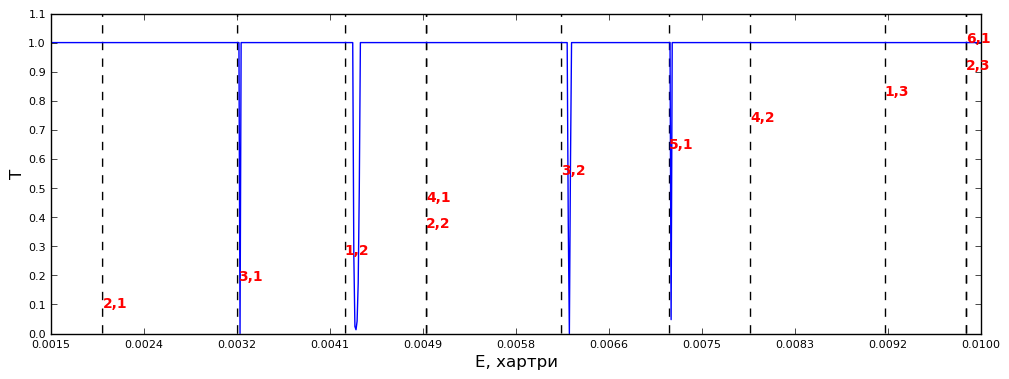
\includegraphics[width=0.8\textwidth]{transmission_all.png}
% \caption{Зависимость коэффициента прохождения от энергии входящей волны. Вертикальные пунктирные линии — собственные энергии резонатора, парами чисел помечены номера соответствующих им собственных состояний.}
% \end{figure}
% \end{frame}

% \begin{frame}[fragile]
% \frametitle{Результаты: коэффициент прохождения в окрестности резонанса}
% \begin{figure}
% 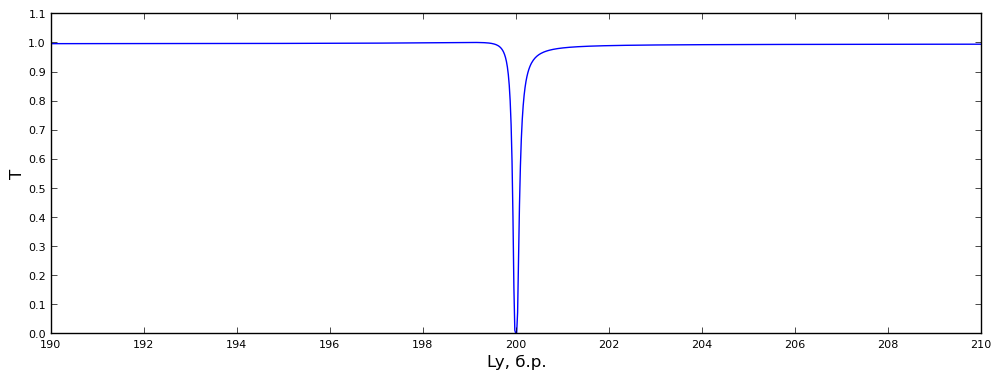
\includegraphics[width=0.8\textwidth]{transmission_size.png}
% \caption{Зависимость коэффициента прохождения от геометрии резонатора}
% \end{figure}
% \end{frame}

\begin{frame}{\todo{Дальнейшие вариации задачи}}
% \begin{easylist}[itemize]
% # Двумерный волновод, квантовая точка внутри проводника
% # Трехмерный волновод, квантовая точка внутри проводника
% # Трехмерный волновод, тороидальный резонатор Гельмгольца
% ## Взаимодействие не точечное, но за счет симметрии может получиться что-то хорошее
% # Полупрозрачная перегородка 
% # Уравнение Дирака
% ## Учитывает релятивистские эффекты
% # Магнитное поле
% \end{easylist}
\end{frame}

\end{document}